% !TeX spellcheck = es
\documentclass{report}
\usepackage[utf8]{inputenc}

% Títulos automáticos en español
\usepackage[spanish]{babel}

% Soporte para buenas urls e hipervínculos entre secciones
\usepackage{hyperref}

% Citas y referencias en formato APA
% Si quiere las citas y referencias en IEEE comente esta línea
\usepackage{apacite}

% Imágenes y figuras
\usepackage{graphicx}

% Código fuente con números de línea
\usepackage{listings}
% Puede cambiar el lenguaje de código fuente
% https://www.overleaf.com/learn/latex/code_listing#Supported_languages
\usepackage{multirow}


\lstset{
    language=C,
    basicstyle=\footnotesize,
    numbers=left,
    stepnumber=1,
    showstringspaces=false,
    tabsize=1,
    breaklines=true,
    breakatwhitespace=false,
}


\def \unidad{Nombre de la escuela o unidad}
\def \programa{Nombre del programa o carrera}
\def \curso{Código - Nombre del curso}
\def \titulo{Título del Informe}
\def \subtitulo {Subtítulo}
\def \autores{
    Nombre del primer autor\\
    Correo electrónico\\
    Carnet\\
    
    \vspace{0.5cm}
    
    Nombre del segundo autor\\
    Correo electrónico\\
    Carnet
}
\def \fecha{Febrero 2021}
\def \lugar{
    Provincia, 
    Costa Rica
}

% Inicia el documento 
\begin{document}

% Inserta la portada del documento
\begin{titlepage}
    \begin{center}
        \vspace*{1cm}
        
        
\includegraphics[width=0.8\linewidth]{figuras/logo_tec.jpg}\\
        \LARGE
        \unidad\\
        \programa\\
        \curso
        
        \vspace{1cm}
        
        \Huge
        \textbf{\titulo}
            
        \vspace{0.5cm}
        \LARGE
        \subtitulo
            
        \vspace{1.5cm}
        
        \large    
        \autores
            
        \vfill
        
        \lugar\\
        \fecha
        
    \end{center}
\end{titlepage}

\tableofcontents

\chapter{Introducción}\label{intro}

Esta es una plantilla para trabajar documentos formales en \LaTeX para informes de trabajos del ITCR, fue diseñada para el curso Fundamentos de Organización de Computadoras.
Esta plantilla utiliza el formato de citas y referencias de APA usando el paquete apacite.

Las tareas y trabajos universitarios deben entregarse en un formato formal que sigan ciertas reglas de estilo. 
\LaTeX es una buena solución para redactar este tipo de documentos sin preocuparse por la estructura ni el diagramado.

\section{Antecedentes}\label{antecedentes}

El matemático y científico en computación Donald Knuth diseñó TeX en 1978 como una respuesta a la necesidad de la época de redactar documentos formales con lenguaje matemático que los editores de texto de la época no podían solventar. En 1984 Leslie Lamport modificó TeX y creó una serie de comandos y macros más sencillos y con más herramientas. A esta versión Lamport le llamó \LaTeX \cite{lopez18}.

\section{Desarrollo}

\subsection{Descripción del proyecto}
El proyecto presentado trata sobre la implementación de un programa de compresión y descompresión de directos de archivos de texto plano. Está diseñado específicamente para la distribución de Debian, pero puede ser ejecutado en otras distribuciones de Linux que compartan las mismas características. La diferencia rige en el archivo de instalación de paquetes necesarios como gcc y make. Sin embargo, estos pueden ser instalados manualmente por el usuario que desee utilizar el programa.

Para realizar las labores de compresión se realiza la utilización del algoritmo de Huffman, éste consiste en tomar las frecuencias de cada conjunto de caracteres presentados en el archivo y crear una lista que los ordene de manera ascendente. Posteriormente se crea el árbol de Huffman, para crearlo se basó en (cap) en donde se realiza la eliminación de los dos primeros nodos de la lista y se agregan a un nuevo nodo que contenga la suma de sus frecuencias. El nodo con menor frecuencia se coloca a la derecha (el primero) y el de mayor frecuencia a la izquierda (el segundo). Luego este nodo se inserta de nuevo a la lista siguiendo el ordenamiento por frecuencia, y así se realiza sucesivamente hasta tener un solo elemento que sería la raíz del árbol.

Una vez creado el árbol se visitan recursivamente los hijos de la raíz para formar el diccionario del código en binario para cada carácter leído de los archivos. Este diccionario se forma concatenando un 0 al código si es que está hacía la derecha del nodo actual o un 1 si está a la izquierda, esto se realiza hasta llegar a un nodo hoja que representaría el carácter buscado.

Con el diccionario formado la compresión del archivo se reduce simplemente a ir reemplazando cada carácter por su equivalente en el archivo de salida objetivo. Para facilitar la descompresión se agrega al inicio del archivo el diccionario formado seguido por el nombre del primer archivo comprimido y la cantidad de bits que este representa. De esta manera, cuando se va a descomprimir se extrae primero el árbol, luego el nombre del archivo junto con su tamaño en bits y posteriormente se realiza la descompresión de dicho archivo, cuando la cantidad de bits reemplazados llegan al total que poseía dicho archivo se estaría cerrando y guardando para procesar el siguiente. Este proceso se realiza repetidamente hasta que no hayan archivos o bits por leer.

\subsection{Instrucciones}
\subsubsection{Cómo instalar el programa}
\begin{enumerate}
  \item Descargue el código fuente del programa. Puede hacerlo de las dos siguientes formas:
    \begin{itemize}
      \item Dirigirse al repositorio de GitHub mediante su navegador a través del siguiente link: \url{https://github.com/Andres2950/SO\_Huffman.git}
      \item Instalarlo directamente con el comando \\
    \texttt{wget \url{https://github.com/Andres2950/SO\_Huffman/archive/refs/heads/main.zip}}
    \end{itemize}
  \item Descomprima el archivo .zip descargado utilizando el comando \texttt{unzip}.
\item Al extraer el archivo podrá observar la estructura de organización mencionada en la sección anterior.
\item Ejecute el archivo \texttt{install.sh}, asegúrese de qué tenga permisos de ejecución, puede utilizar el comando \texttt{chmod +x install.sh} en caso de que no los posea y luego ejecute de la siguiente forma \texttt{./install.sh}. \\
  Este archivo se hará cargo de la instalación del compilador \textit{gcc} necesario para compilar el código fuente. Además hará la instalación del paquete \textit{make} para la ejecución de archivos makefile, dicho archivo posee las instrucciones de compilación de \textit{gcc} para resolver todas las dependencias que se encuentran en el directorio \textit{src/headers}.  
\item Note que la instalación de dichos paquetes requiere permisos de usuarios root, al ejecutar el archivo \texttt{install.sh} este se volverá a ejecutar con dichos permisos, para esto solicitará la contraseña del usuario root para tener dichos permisos de ejecución (la contraseña es totalmente invisible para el programa) y así poder descargar los paquetes. Mostrará un mensaje como el de la figura N y esperará la entrada correcta.
\item La compilación de los archivos se realiza sin permisos root.
\item Además, el \texttt{install.sh} hará una copia de los binarios \texttt{huff} y \texttt{dehuff} en el directorio \textit{/usr/bin} de la máquina para poner ser accedidos desde cualquier lugar y utilizado en múltiples directorios sin necesidad de mover los archivos a comprimir o descomprimir a una carpeta en particular.

\end{enumerate}

\subsubsection{Cómo utilizar el programa}
Una vez terminado el procedimiento de instalar el programa puede utilizar el comando huff para comprimir archivos. Dicho comando posee una serie de parámetros para sus distintos modos de ejecución. A continuación se detallan cada uno.
\begin{itemize}
  \item \textbf{huff -h}\\ \hspace{2cm}
    Provee una guía de los parámetros requeridos por el programa y su orden de entrada. (Véase figura N)
  \item \textbf{huff [Opción] src dst} o \textbf{dehuff [Opción] src dst}\\
src es el directorio objetivo a ser comprimido/descomprimido\\
dst es el archivo de destino
  \item \textbf{Opciones} 
    \begin{itemize}
      \item \textbf{-s} modo de ejecución serial.
      \item \textbf{-p} modo de ejecución paralela usando fork.
      \item \textbf{-c} modo de ejecución concurrente usando pthread
      \item \textbf{-b} modo de Benchmark para comparar los tiempos de ejecuión entre los anteriores modos.
    \end{itemize}
\end{itemize}





\section{Discusión}
\subsection{Resultados de las pruebas}
\subsubsection{Metodología de las pruebas}

Las pruebas que se realizaron tenían el objetivo de obtener el tiempo de ejecución del programa o una parte de este. Para lograr esto se decidió tomar marcas de tiempo en el código al inicio y al final de la parte que se quería probar. Se utilizó el header time.h tomar los tiempos. El tiempo de ejecución  se imprime en pantalla como la diferencia entre las dos marcas de tiempo.

Se realizaron pruebas en distintas partes de los programas y cada prueba se realizó en las 3 implementaciones diferentes. En total se probó el sistema completo del compresor y sus subsistemas de lectura y compresión; y el sistema completo del descompresor y su subsistema de descompresión y escritura.

Cada prueba se ejecutó 50 veces de forma independiente. La tabla de resultados contiene el promedio de las 50 pruebas.

\subsubsection{Tabla de resultados}

\begin{center}
	\begin{tabular}{|c|c|c|c|}		
		
\hline
\multicolumn{4}{|c|}{Tiempo de Ejecución (milisegundos)} \\
\hline
 Subsistema& \multicolumn{3}{|c|}{Versión} \\
 \hline
 & Serial & Concurrente & Paralelo\\
 \hline
huff(completo) & 5360& 2226 & 2036\\
 \hline
huff(lectura) &  36 & 25 & 19\\
 \hline
 huff(compresión) &  5168 & 1957 & 1681\\
 \hline
 dehuff(completo) & 5189 & 2092 & 1855\\
 \hline
 dehuff(descompresión y escritura) & 5146 & 1968 & 1629\\
 \hline
 
	\end{tabular}
\end{center}

\subsection{Análisis de aceleración}

\subsubsection{Metodología de Análisis}

Gene Amdahl (1922–2015) fue un informático especializado en arquitectura de hardware. Su contribución más conocida a la informática es su ley homónima, propuesta en 1967. 

La ley de Amdahl modela cuánto puede mejorarse el rendimiento del sistema al paralelizar el código. Muestra que, incluso con una potencia de cálculo infinita, las partes secuenciales limitan la aceleración. Esta ley ayuda a los desarrolladores a estimar las mejoras de rendimiento y a optimizar las secciones de código de alto impacto. La fórmula que representa la ley es la siguiente:



\begin{displaymath}	
	{T_{m} = {T_{a} \cdot \left((1 - F_{m}) + {F_{m} \over A_{m}}\right)}}
\end{displaymath}

Esta fórmula puede reescribirse para obtener la aceleración de un sistema completo luego de que se optimiza un subsistema. La formula sería la siguiente:

\begin{displaymath}	
	A = {1 \over (1 - F_{m}) + {F_{m} \over A_{m}}}	
\end{displaymath}
Donde:\\
$A$, es la aceleración o ganancia en velocidad conseguida en el sistema completo debido a la mejora de uno de sus subsistemas.\\
$A_{m}$, es el factor de mejora que se ha introducido en el subsistema mejorado.\\
$F_{m} $, es la fracción de tiempo que el sistema utiliza el subsistema mejorado.\\

La ley de Amdahl muestra que hay un limite en la aceleración posible que se puede obtener optimizando un programa. La siguiente re escritura de la fórmula nos da la aceleración máxima teórica para un sistema cuando N tiende a infinito.

	\begin{displaymath}	
		A = {2 \cdot \left 1 \over  S + {1-S \over N}}
	\end{displaymath}
Donde:\\
$A$, es la aceleración máxima conseguida en el sistema completo debido a la mejora de uno de sus subsistemas.\\
$S$, es la fracción del programa que es secuencial.\\
$N$,  el factor de mejora.\\

En las próximas secciones se realiza el cálculo par obtener la mejora de los programas de compresión y descompresión luego de haber sido optimizados mediante paralelización y concurrencia. Además se hace una discusión sobre las ganancias obtenidas a través de los diferentes métodos.

\subsubsection{Aceleración del compresor(huff)}

La ejecución del compresor se puede dividir en 3 fases: lectura, creación del árbol huffman, compresión y escritura. La etapa de lectura es donde se lee cada uno de los archivos del directorio fuente, esta etapa puede ser paralelizada.  La etapa de creación del  árbol huffman es donde se junta todo el texto para crear el diccionario con el código huffman, esta etapa no puede ser paralelizada. La etapa de compresión corresponde a la transformación de texto plano a codigo huffman de cada uno de los archivos, esta etapa puede ser paralelizada. La etapa de escritura es donde se escribe el código de cada archivo a un documento binario, esta etapa puede ser paralelizada pero se decidió no hacerlo.

La fracción del programa que abarca cada etapa sería: lectura(0.06), compresión(0.964), creación de árbol y escritura(0.02).  Lo que quiere decir que un 98\% del programa puede paralelizarse, esto implica que la aceleración máxima teórica del programa sería de 100.

La aceleración máxima que se logra obtener mediante el uso de hilos es de 2.341 y mediante el uso de fork es de 2.549. 

Ambas implementaciones mejoran drásticamente el tiempo de ejecución del programa. Ninguno de los dos se acercan al máximo teórico debido al overhead que tiene la paralelización, además el compresor cuenta con un cuello de botella en la etapa de creación del árbol huffman que se encuentra justo entre las dos etapas que se paralelizaron, lo que obliga el programa  a paralelizarse y serializarse dos veces.

Se puede observar que la implementación con paralela  fork es ligeramente más rápida que la  concurrente con hilos.

\subsubsection{Aceleración del descompresor(dehuff)}

La ejecución del descompresor se puede dividir en 2 fases: lectura del diccionario y reconstrucción del árbol, y descompresión y escritura. La primera etapa es donde se lee el inicio del archivo comprimido donde se encuentra el diccionario de códigos y se reconstruye el árbol en base a este, esta etapa no puede paralelizarse. La última etapa corresponde a la lectura del codigo de cada archivo, su descompresión y escritura, esta etapa puede ser paralelizada. 

La fracción del programa que abarca cada etapa sería: lectura de diccionario y reconstrucción de árbol (0.01), y descompresión y escritura(0.99).  Lo que quiere decir que un 99\% del programa puede paralelizarse, esto implica que la aceleración máxima teórica del programa sería de 200.

La aceleración máxima que se logra obtener mediante el uso de hilos es de 2.444 y mediante el uso de fork es de 2.727 

Ambas implementaciones mejoran drásticamente el tiempo de ejecución del programa. Ninguno de los dos se acercan al máximo teórico debido al overhead que tiene la paralelización.

 Se puede resaltar que el compresor y el descompresor tienen una fracción virtualmente idéntica de sus sistemas que fue paralelizado. Sin embargo, el descompresor obtuvo una mejor aceleración, indiferente de la implementación. Esto puede deberse a que descompresor realiza todas las tareas paralelas en el mismo punto en el código, sin ningún cuello de botella.

Se puede observar que la implementación paralela con fork es ligeramente más rápida que la  concurrente con hilos.


\chapter{Ejemplos}\label{ejemplos}

\section{Figuras}\label{figuras}
\begin{figure}
    \centering
    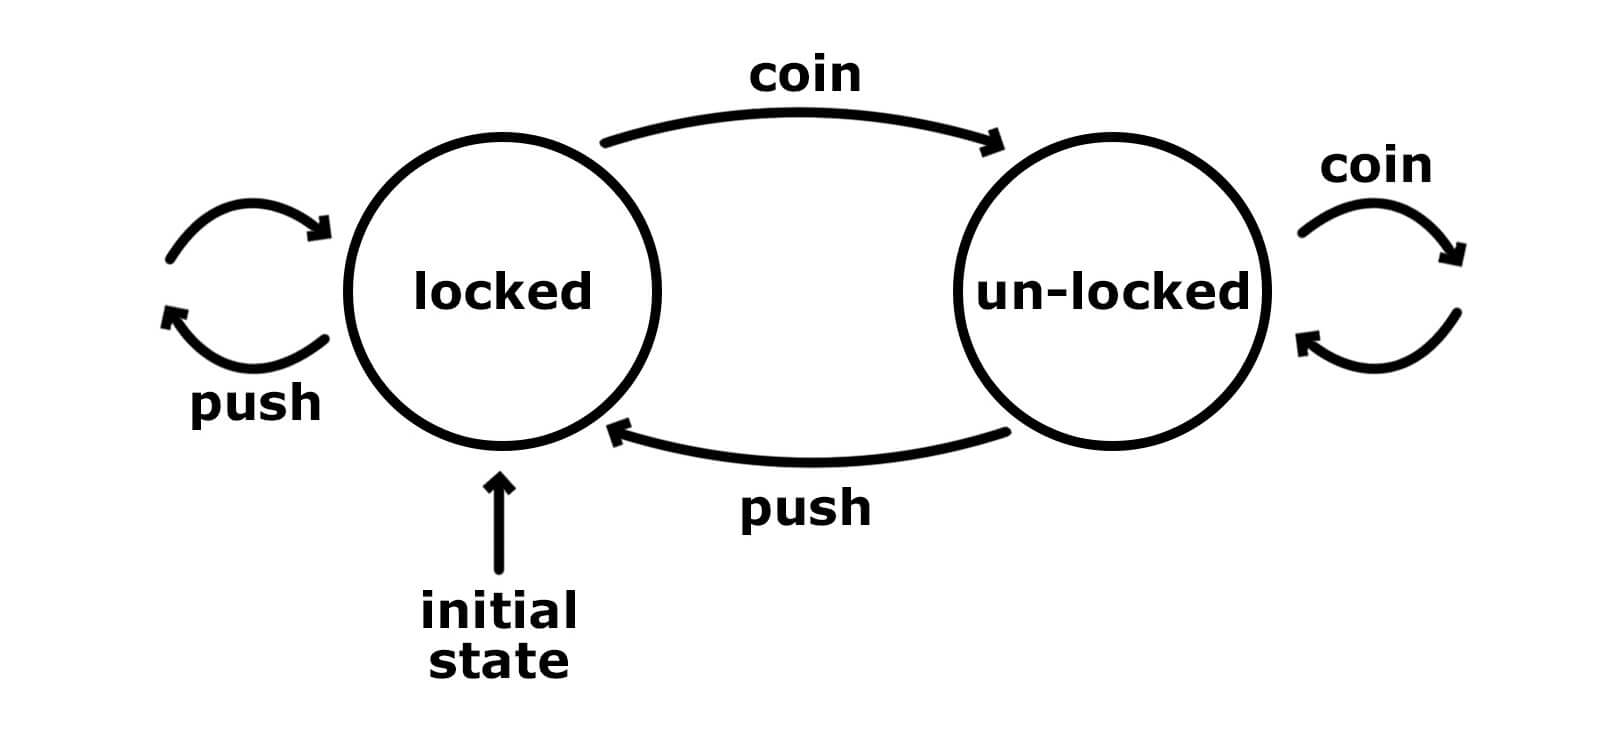
\includegraphics[width=0.8\linewidth]{figuras/maquinaDeEstados.jpg}
    \caption{Ilustración de una máquina de estados finitos}
    \label{fig:msf}
\end{figure}

Las figuras nos permiten ilustrar conceptos de forma más directa. Adicionalmente muchos dominios emplean lenguajes gráficos para representar ciertos principios o procesos. La figura permite incorporar este tipo de herramientas visuales al documento. 
La figura \ref{fig:msf} representa una máquina de estados finitos, nótese como la figura incorpora un texto descriptivo. Este texto es necesario para brindar mejor contexto a la imagen, especialmente cuando no se diagrama junto al texto que acompaña.

\section{Listas y Enumeraciones}\label{listas}

Las listas de viñetas y enumeraciones nos permiten organizar información y secuenciarla de forma visualmente agradable. Bien empleadas las listas pueden ayudar a organizar los datos presentados y establecer cierta noción de jerarquía.

Una lista puede contener solamente algunos elementos simples:
\begin{itemize}
    \item ítem 1
    \item ítem 2
    \item ítem 3
\end{itemize}

Pero también se pueden emplear de formas más complejas e interesantes:

\begin{itemize}
    \item \textbf{Conceptos amplios:} Por ejemplo una lista puede usarse para representar ideas más complejas que pueden organizarse en algún tipo de jeraruía. 
    Una lista de este tipo puede contener mucho texto, párrafos inclusive, y aún así mantener la indentación y estructura lineal que permite expresar la relación como parte de la información transmitida.
    
    Los elementos de la lista se pueden introducir con un encabezado en \textbf{negrita} que permita asociar los conceptos con sus definiciones. Similar a las entradas de un diccionario.
    
    \item \textbf{Contenido multinivel:} Otra aplicación de las listas es que permiten organizar contenido en estructuras jerárquicas. En \LaTeX una lista puede:
    
    \begin{itemize}
        \item Anidarse dentro de otra lista
        \item Mostrando múltiples elementos
        \item Dentro de una estructura jerárquica
        \begin{itemize}
            \item Tan profunda
            \item Como el autor
            \item Lo requiera
        \end{itemize}
    \end{itemize}
\end{itemize}

Por supuesto si podemos hacer listas de viñetas, \LaTeX también nos da la posibilidad de usar enumeraciones:

\begin{enumerate}
    \item Las enumeraciones tienen las mismas propiedades.
    \item La única diferencia es que los ítemes se identifican con números, no con viñetas.
    \item Pero soportan:
    \begin{enumerate}
        \item texto corto
        \item texto largo
        \item multinivel
        \item Inclusive es posible combinar ambas estrategias:
        \begin{itemize}
            \item Enumeraciones con listas adentro
            \item Listas con enumeraciones adentro
            \item Cualquier otra combinación que sea necesaria
            
        \end{itemize}
    \end{enumerate}
\end{enumerate}

\section{Referencias Internas}\label{referencias}
En el capítulo \ref{intro} se explica el propósito del documento y algunos antecedentes. Mientras que el capítulo \ref{ejemplos} se enfoca más en funcionalidades puntuales que pueden ser interesantes de \LaTeX. Como se puede apreciar, una de esas funcionalidades es la capacidad de referenciar internamente contenido, usando los comandos \textit{label} y \textit{ref} es posible citar otras partes del documento. Cualquier elemento numerado con una \textbf{etiqueta} se puede referenciar y \LaTeX usará la numeración correcta para referenciar el elemento donde se cite. Por ejemplo en esta sección se puede citar la figura \ref{fig:msf} o la sección \ref{antecedentes}. Una propiedad muy práctica de esta herramienta, es que combinada con el paquete \textbf{hyperref} permite que el documento se entrelace fácilmente, creando hipervínculos entre las secciones justo donde se referencian.

Nótese que estas son referencias internas. Las citas bibliográficas tienen un comando especial: el comando \textbf{cite}.

\section{Código fuente}
En temas de ingeniería es normal que necesitemos programar de vez en cuando. Para esto \LaTeX brinda funcionalidades para renderizar código fuente con un resultado bastante profesional.
Por ejemplo podemos ver el código fuente de un \textit{Hola Mundo} en el lenguaje de programación C:

\begin{lstlisting}
#include <stdio.h>

int main() {
   
   printf("Hello, World!");
   return 0;
}
\end{lstlisting}

Hay más herramientas para mostrar texto técnico. Por ejemplo el ambiente \textit{verbatim} permite mostrar texto con símbolos que normalmente están reservados para código de \LaTeX. Por ejemplo, estas son las primeras líneas de este documento:

\begin{verbatim}
\documentclass{report}
\usepackage[utf8]{inputenc}

% Títulos automáticos en español
\usepackage[spanish]{babel}

% Soporte para buenas urls e hipervínculos entre secciones
\usepackage{hyperref}
\end{verbatim}

\section{Más}
\LaTeX tiene muchísimas características, tantas que es imposible cubrirlas todas en un sólo documento. Por eso voy a dejar una lista breve de algunos enlaces de interés que podrían ser útiles según el tipo de documento:

\begin{itemize}
    \item \textbf{Tablas:} \\
    \url{https://manualdelatex.com/tutoriales/tablas}
    
    \item \textbf{Bibliografía con Bibtex:}\\
    \url{https://www.overleaf.com/learn/latex/bibliography_management_with_bibtex}
    
    \item \textbf{Expresiones Matemáticas:}\\
    \url{http://metodos.fam.cie.uva.es/~latex/apuntes/apuntes3.pdf}
    
    \item \textbf{Presentaciones de Diapositivas:}\\
    \url{https://www.overleaf.com/learn/latex/beamer}
    
    \item \textbf{Gráficas generadas en \LaTeX}\\
    \url{https://www.overleaf.com/gallery/tagged/charts}    
\end{itemize}

% Estilo de bibliografía APA
% Si quiere usar el estilo IEEE comente esta línea
\bibliographystyle{apacite}

% Descomente esta línea para usar el estilo de bibliografía IEEE
%\bibliographystyle{ieeetr}
\bibliography{referencias}

\end{document}
